\section{Date: 2026-07-31}
\noindent \textbf{Series ID: GLAKPCEPCFININS} 

\noindent This series is titled Per Capita Personal Consumption Expenditures: Services: Financial Services and Insurance for Great Lakes BEA Region and has a frequency of Annual. The units are Dollars and the seasonal adjustment is Not Seasonally Adjusted.The observation start date is 1997-01-01 and the observation end date is 2024-01-01.The popularity of this series is 1. \\ 

\noindent \textbf{Series ID: DICISYPIMEPS} 

\noindent This series is titled Medical Services Expenditures by Disease: Diseases of the Circulatory System Price Index, MEPS Account Basis and has a frequency of Annual. The units are Index 2017=100 and the seasonal adjustment is Not Seasonally Adjusted.The observation start date is 2000-01-01 and the observation end date is 2021-01-01.The popularity of this series is 2. \\ 

\subsection{Raw Regression}
\noindent Regresses the two series against each other directly. A significant result here can come just as easily from both series sharing a long-run trend as from any real relationship.

\begin{center}
\begin{tabular}{lclc}
\toprule
\textbf{Dep. Variable:}               & value\_fred\_DICISYPIMEPS & \textbf{  R-squared:         } &     0.455   \\
\textbf{Model:}                       &            OLS            & \textbf{  Adj. R-squared:    } &     0.428   \\
\textbf{Method:}                      &       Least Squares       & \textbf{  F-statistic:       } &     16.70   \\
\textbf{Date:}                        &      Fri, 31 Jul 2026     & \textbf{  Prob (F-statistic):} &  0.000574   \\
\textbf{Time:}                        &          13:24:03         & \textbf{  Log-Likelihood:    } &   -68.826   \\
\textbf{No. Observations:}            &               22          & \textbf{  AIC:               } &     141.7   \\
\textbf{Df Residuals:}                &               20          & \textbf{  BIC:               } &     143.8   \\
\textbf{Df Model:}                    &                1          & \textbf{                     } &             \\
\textbf{Covariance Type:}             &         nonrobust         & \textbf{                     } &             \\
\bottomrule
\end{tabular}
\begin{tabular}{lcccccc}
                                      & \textbf{coef} & \textbf{std err} & \textbf{t} & \textbf{P$> |$t$|$} & \textbf{[0.025} & \textbf{0.975]}  \\
\midrule
\textbf{const}                        &      79.4286  &        5.232     &    15.181  &         0.000        &       68.515    &       90.343     \\
\textbf{value\_fred\_GLAKPCEPCFININS} &       0.0083  &        0.002     &     4.087  &         0.001        &        0.004    &        0.013     \\
\bottomrule
\end{tabular}
\begin{tabular}{lclc}
\textbf{Omnibus:}       &  0.906 & \textbf{  Durbin-Watson:     } &    1.079  \\
\textbf{Prob(Omnibus):} &  0.636 & \textbf{  Jarque-Bera (JB):  } &    0.253  \\
\textbf{Skew:}          &  0.253 & \textbf{  Prob(JB):          } &    0.881  \\
\textbf{Kurtosis:}      &  3.142 & \textbf{  Cond. No.          } & 1.09e+04  \\
\bottomrule
\end{tabular}
%\caption{OLS Regression Results}
\end{center}

Notes: \newline
 [1] Standard Errors assume that the covariance matrix of the errors is correctly specified. \newline
 [2] The condition number is large, 1.09e+04. This might indicate that there are \newline
 strong multicollinearity or other numerical problems.

\begin{figure}
\centering
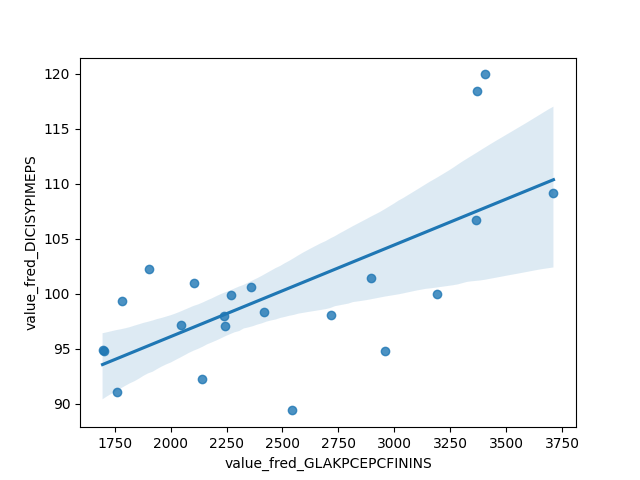
\includegraphics[scale = 0.9]{plots/plot_2026-07-31.png}
\caption{Raw Regression Plot for 2026-07-31}
\end{figure}
\newpage
\subsection{Detrended Regression}
\noindent Regresses the residuals of each series after removing its own linear time trend, so a shared trend can no longer drive the result on its own. A relationship that stays significant here is better evidence of a genuine link between the two series.

\begin{center}
\begin{tabular}{lclc}
\toprule
\textbf{Dep. Variable:}                          & value\_fred\_DICISYPIMEPS\_detrended & \textbf{  R-squared:         } &     0.077   \\
\textbf{Model:}                                  &                 OLS                  & \textbf{  Adj. R-squared:    } &     0.030   \\
\textbf{Method:}                                 &            Least Squares             & \textbf{  F-statistic:       } &     1.657   \\
\textbf{Date:}                                   &           Fri, 31 Jul 2026           & \textbf{  Prob (F-statistic):} &    0.213    \\
\textbf{Time:}                                   &               13:24:03               & \textbf{  Log-Likelihood:    } &   -68.753   \\
\textbf{No. Observations:}                       &                    22                & \textbf{  AIC:               } &     141.5   \\
\textbf{Df Residuals:}                           &                    20                & \textbf{  BIC:               } &     143.7   \\
\textbf{Df Model:}                               &                     1                & \textbf{                     } &             \\
\textbf{Covariance Type:}                        &              nonrobust               & \textbf{                     } &             \\
\bottomrule
\end{tabular}
\begin{tabular}{lcccccc}
                                                 & \textbf{coef} & \textbf{std err} & \textbf{t} & \textbf{P$> |$t$|$} & \textbf{[0.025} & \textbf{0.975]}  \\
\midrule
\textbf{const}                                   &   -2.898e-12  &        1.232     & -2.35e-12  &         1.000        &       -2.569    &        2.569     \\
\textbf{value\_fred\_GLAKPCEPCFININS\_detrended} &       0.0115  &        0.009     &     1.287  &         0.213        &       -0.007    &        0.030     \\
\bottomrule
\end{tabular}
\begin{tabular}{lclc}
\textbf{Omnibus:}       &  0.853 & \textbf{  Durbin-Watson:     } &    1.130  \\
\textbf{Prob(Omnibus):} &  0.653 & \textbf{  Jarque-Bera (JB):  } &    0.357  \\
\textbf{Skew:}          &  0.312 & \textbf{  Prob(JB):          } &    0.836  \\
\textbf{Kurtosis:}      &  2.997 & \textbf{  Cond. No.          } &     138.  \\
\bottomrule
\end{tabular}
%\caption{OLS Regression Results}
\end{center}

Notes: \newline
 [1] Standard Errors assume that the covariance matrix of the errors is correctly specified.

\begin{figure}
\centering
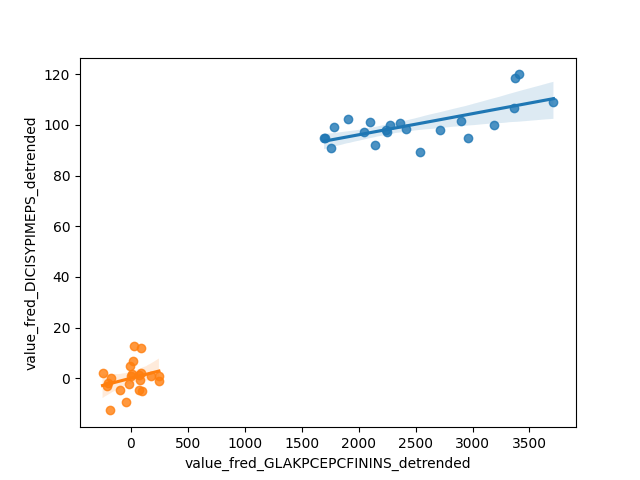
\includegraphics[scale = 0.9]{plots/plot_2026-07-31_detrended.png}
\caption{Detrended Regression Plot for 2026-07-31}
\end{figure}
\newpage
